\Problem{Polyomino Powers}{polyomino}
% author: Andreas Bj\"orklund

\begin{wrapfigure}{r}{7cm}
\vspace{-5mm}
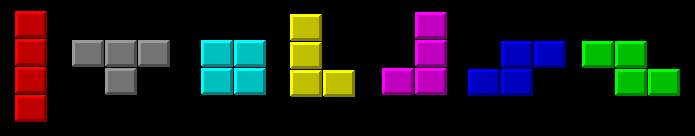
\includegraphics[width=\linewidth,keepaspectratio=true]{polyomino/TetrisPieces}
\vspace{-9mm}
\end{wrapfigure}

\noindent
A polyomino is a polyform with the square as its base form. It is a
connected shape formed as the union of one or more identical squares in
distinct locations on the plane, taken from the regular square tiling,
such that every square can be connected to every other square through a
sequence of shared edges (i.e., shapes connected only through shared
corners of squares are not permitted). \\
The most well-known polyominos are the seven tetrominos made out of four squares (see figure),
famous from the Tetris$^{\textregistered}$ game, and of course the single domino consisting of two squares
from the game with the same name. Some polyomino can be obtained by
gluing several copies of the same smaller polyomino translated (but not rotated or mirrored) to different locations in the plane.
We call those polyomino powers.\\

\Input
One line with two positive integers $h, w \leq 10$. \\
Next follows an $h \times w$ matrix of characters '.' or 'X', the 'X''s describing a polyomino and '.' space.

\Output
A $k$-power with $2 \leq k \leq 5$ copies of a smaller polyomino: \\
Output a $h\times w$ matrix on the same format as the input with the 'X''s replaced by the numbers $1$ through $k$ in any order identifying the factor pieces. \\
Furthermore, if multiple solutions exist, any will do. Otherwise, output 'No solution' if no solution exists.

\Xample{polyomino/polyomino.1}

\Xample{polyomino/polyomino.2}

\Xample{polyomino/polyomino.3}
